
\section{Comparing the Non Relativistic and Relativistic Results}
    \begin{figure}[h]
    \begin{center}
    \begin{tabular}{cc}
        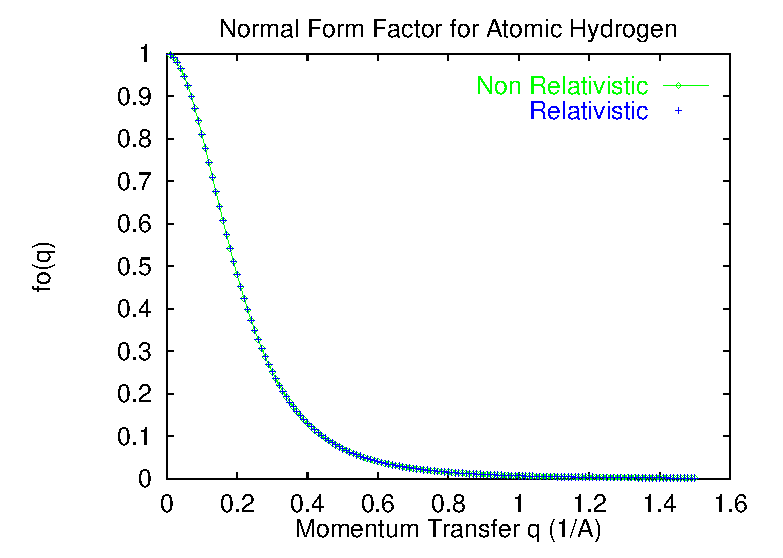
\includegraphics[width=7.0cm]{f0_hydrogen.eps}
        &
        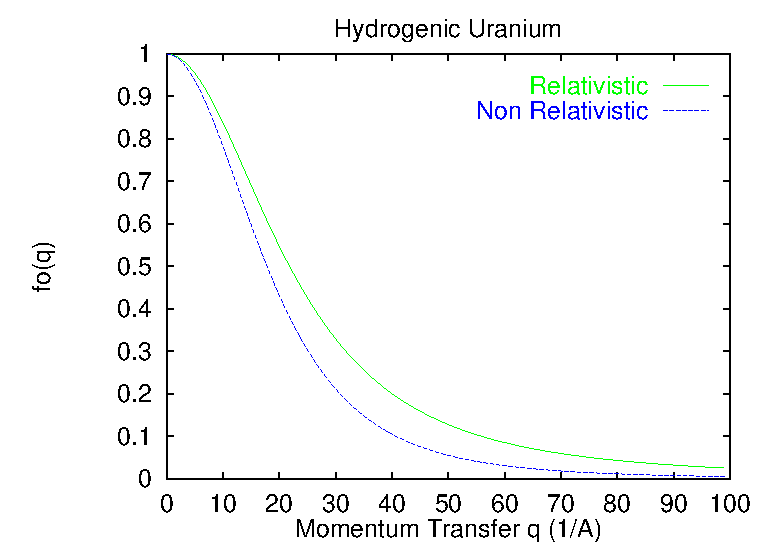
\includegraphics[width=7.0cm]{f0_uranium.eps}
    \end{tabular}
    \caption{Normal Form Factor for Single Electron Hydrogen and Uranium}
    \label{fig:hydrogen-uranium}
    \end{center}
    \end{figure}
    The relativistic normal form factor in equation~\ref{eq:nff-relativistic}
    can be compared to the non relativistic case by considering the small values
    of $Z$ in which the parameter $\gamma_1 = \sqrt{1-\alpha^2Z^2} \approx 1$. 
    In this case equation~\ref{eq:nff-relativistic} becomes:
    \begin{equation} \label{eq:reduction}
        f_0(q) \approx 
        2 \frac{\Gamma(2)}{\Gamma(3)}
        \left( \frac{2Z}{a_0} \right)^4
        \left[ 
            \left( \frac{2Z}{a_0} \right)^2 + q^2
        \right]^{-2} 
        =
        \left( \frac{2Z}{a_0} \right)^4
        \left[ 
            \left( \frac{2Z}{a_0} \right)^2 + q^2
        \right]^{-2} 
    \end{equation}
    which is in agreement with equation~\ref{eq:nff-nonrelativistic}.
    In figure~\ref{fig:hydrogen-uranium} we see plots for $f_0(q)$ comparing the non relativistic
    and relativistic results for standard atomic hydrogen and hydrogenic
    uranium.
    We can see that in the case of atomic hydrogen ($Z=1$), there is
    excellent agreement between the two results.
    In the case of hydrogenic uranium ($Z=92$) we can see that there is a
    significant difference over a range of momentum transfers between the
    relativistic and non relativistic results. 
    This shows the need for using relativistic Dirac wave functions as opposed to
    the Schr\"odinger wave functions when computing atomic form factors
    especially for heavier atoms.
    In figure~\ref{fig:hydrogen-uranium} it is difficult to make out difference
    between relativistic and non relativistic values for atomic hydrogen, since
    there seems to be quite good agreement between the two. However, if we plot
    the difference between the two results as is done in
    figure~\ref{fig:delta-theory}, we can clear identify the regions of momentum
    transfer where the relativistic theory is better even though the difference
    is of the order of $10^{-6}$ or less. We can see that the maximum
    difference between the two theories is at approximately $q = 0.3 \InvAngstrom$ and
    and it gets smaller at higher values of $q$.
    \begin{figure}[h]
    \begin{center}
        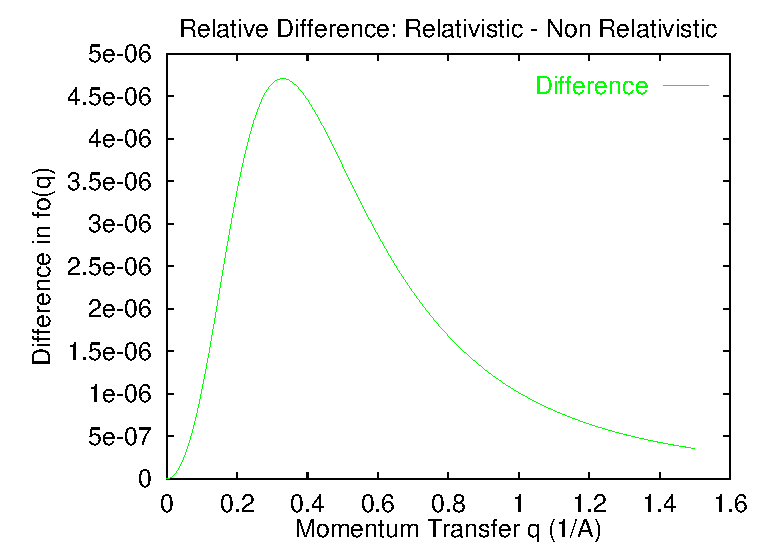
\includegraphics[width=7.0cm]{delta_theory.eps}
        \caption{Difference ($\Delta f_0(q)$) between relativistic and non relativistic theory}
        \label{fig:delta-theory}
    \end{center}
    \end{figure}

\section{Comparison with other theoretical results}
    \begin{figure}[H] 
    \begin{center}
    \begin{tabular}{cc}
        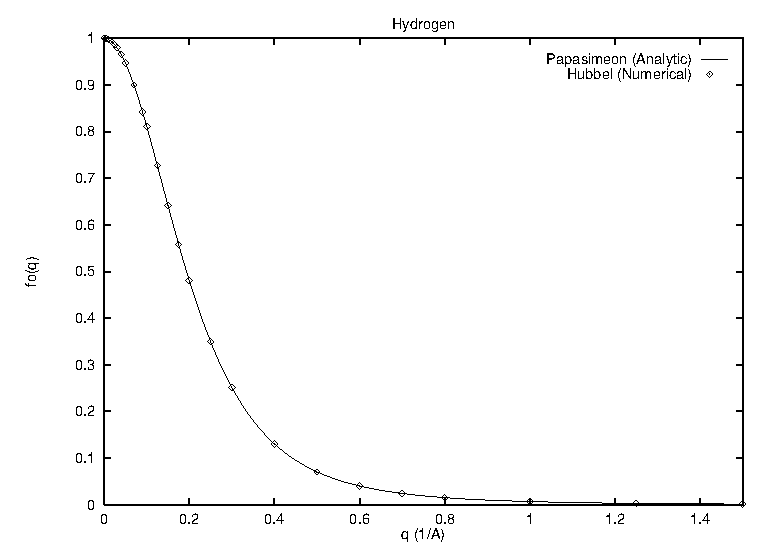
\includegraphics[width=7.0cm]{hubbel_papa.eps}
        &
        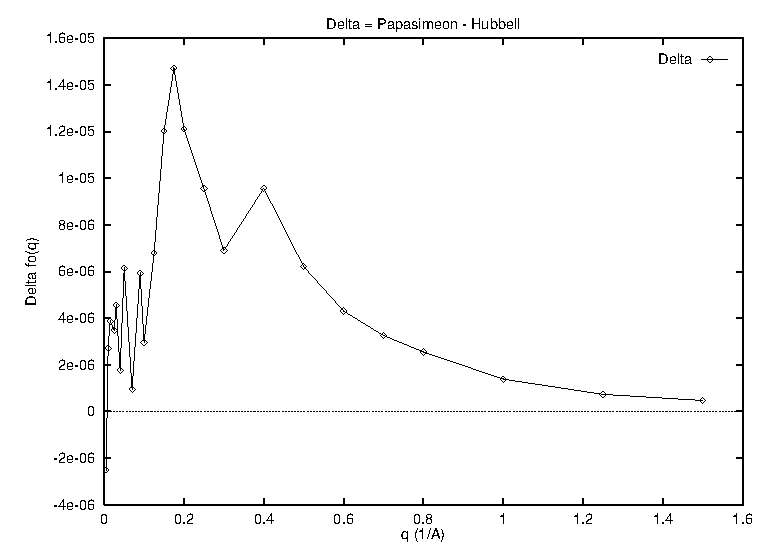
\includegraphics[width=7.0cm]{delta_hubbell.eps}
    \end{tabular}
        \caption{Normal Form Factor for Hydrogen -- Comparison With Hubbell's Theoretical Results}
        \label{fig:hubbell-comparison}
    \end{center}
    \end{figure}
    We can make a comparison between the results obtained using equation~\ref{eq:nff-relativistic}
    and other theoretical results which have used relativistic wave functions in
    computing $f_0(q)$.
    Tabulations of atomic form factors, incoherent scattering function and
    photon scattering cross sections were published by Hubbel et.  al.~\cite{Hubbell-1975}.
    The tabulations for the normal form factor for hydrogen used non
    relativistic wave functions. Figure~\ref{fig:hubbell-comparison} shows two
    plots comparing the analytic result of equation~\ref{eq:nff-relativistic} with
    Hubbel's tabulated results. The plot on the left shows good agreement, but
    looking at the difference between the two theories on the plot on the right
    shows the differences more clearly. The shape is similar to that shown
    in figure~\ref{fig:delta-theory} but the maximum difference is of the order
    of $10^{-5}$.
